% robustness.tex

%%%%%%%%%%%%%%%%%%%%
\begin{frame}{What is Robustness?}
	数据库鲁棒性常被分为动态鲁棒性和静态鲁棒性两个层次来讨论。

	\begin{itemize}
		\item 动态鲁棒性研究数据库的某一个弱隔离级别 $I_1$ 下的执行历史 $H$ 是否满足较强的隔离级别 $I_2$(一般是 SER)。如果满足,我们说 $H$ 在 $I_1$ 下是鲁棒的。动态鲁棒性的研究与执行历史验证较为相似。
		\item 静态鲁棒性研究客户程序 $P$ 在弱隔离级别 $I_1$ 下的所有执行历史是否都满足较强的隔离级别 $I_2$(一般是 SER)。如果满足,我们说 $P$ 在 $I_1$ 下是鲁棒的。例如,如果 $P$ 在 SI 下鲁棒,则我们可以在 SI 下运行 $P$,这可以在保证执行历史满足 SER 的情况下提高系统性能和吞吐率。
	\end{itemize}
\end{frame}
%%%%%%%%%%%%%%%%%%%%

%%%%%%%%%%%%%%%%%%%%
\begin{frame}{State of the Art}
	\begin{table}[]
\centering
\caption{$I_{1} \setminus I_{2}:$ Robustness against $I_{1}$ relative to $I_{2}$.}
\renewcommand{\arraystretch}{1.8}
\resizebox{\textwidth}{!}{%
\begin{tabular}{|c||c|c|c|}
	\hline
	$I_1 \setminus I_2$ & \pc & \si & \ser
	\\ \hline\hline
	\ru & & & [Ketsman PODS'2020] (非分布式)充要条件
	\\ \hline
	\rc & & & \incell{[Ketsman PODS'2020] (非分布式)充要条件}{[Vandevoort VLDB'2021] (非分布式)事务模板充要条件}
	\\ \hline
	\ra & & &
	\\ \hline
	\cc & [Bouajjani ESOP'2021] 充要条件
			& [Bouajjani ESOP'2021] 充要条件
			& \incell{[Bernardi CONCUR'2016] 充分条件}{[Beillahi CONCUR'2019] 充要条件}
	\\ \hline
	\pc & / & [Bouajjani ESOP'2021] 充要条件
		  & [Bernardi CONCUR'2016] 充分条件
	\\ \hline
	\psiso & / & [Cerone PODC'2016] 充分条件
				 & [Bernardi CONCUR'2016] 充分条件
	\\ \hline
	\si  & / & / & \incell{[Fekete TODS'2005] 充分条件}{\incell{[Cerone PODC'2016\&JACM'2018] 充分条件}{[Bernardi CONCUR'16] 充分条件}}
	\\ \hline
\end{tabular}
}
\end{table}
\end{frame}
%%%%%%%%%%%%%%%%%%%%

%%%%%%%%%%%%%%%%%%%%
\begin{frame}{TODS2025 Allocating Isolation Levels to Transactions in a Multiversion Setting}
	\begin{columns}
		\begin{column}{0.5\textwidth}
			\textbf{Problems: }开发人员手动为每类的事务选择隔离级别具有挑战性。选择过于保守,会严重影响吞吐量;选择较低的隔离级别,则需要复杂的并发逻辑来避免异常。

			\textbf{Contributions: }一种在多版本数据库中系统性地分配隔离级别给事务的框架,能够根据事务行为,自动分配最合适的隔离级别,在确保在所需正确性的前提下最大化性能。
		\end{column}
		\begin{column}{0.5\textwidth}
			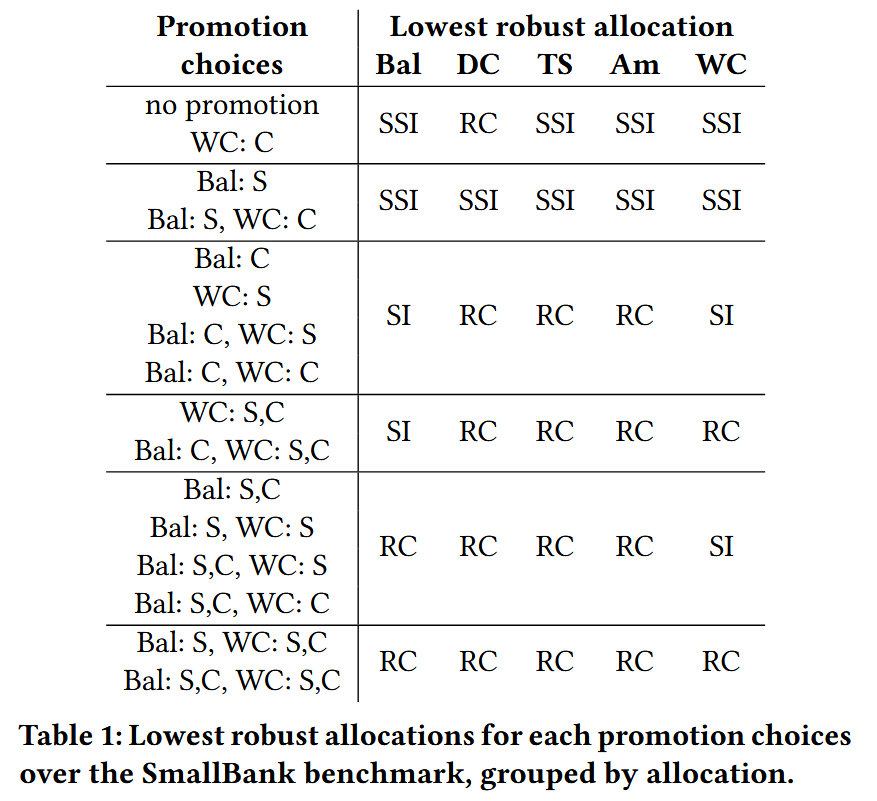
\includegraphics[width=0.98\linewidth]{figs/lowest-robust-allocations}
		\end{column}
	\end{columns}
\end{frame}
%%%%%%%%%%%%%%%%%%%%

%%%%%%%%%%%%%%%%%%%%
\begin{frame}{TODS2025 Allocating Isolation Levels to Transactions in a Multiversion Setting}
	\begin{columns}
		\begin{column}{0.5\textwidth}
			\textbf{Techniques (basic ideas): }分析事务的访问模式(读集和写集),动态识别潜在的冲突依赖环:
			\begin{itemize}
				\item 对只读事务,安全分配 RC 以实现高吞吐量;
				\item 对可能产生依赖环的事务,自动提升隔离级别至 SI 或 SER;
				\item 结合静态分析与运行时监控,在事务执行前/期间动态决策隔离级别。
			\end{itemize}
		\end{column}
		\begin{column}{0.5\textwidth}
			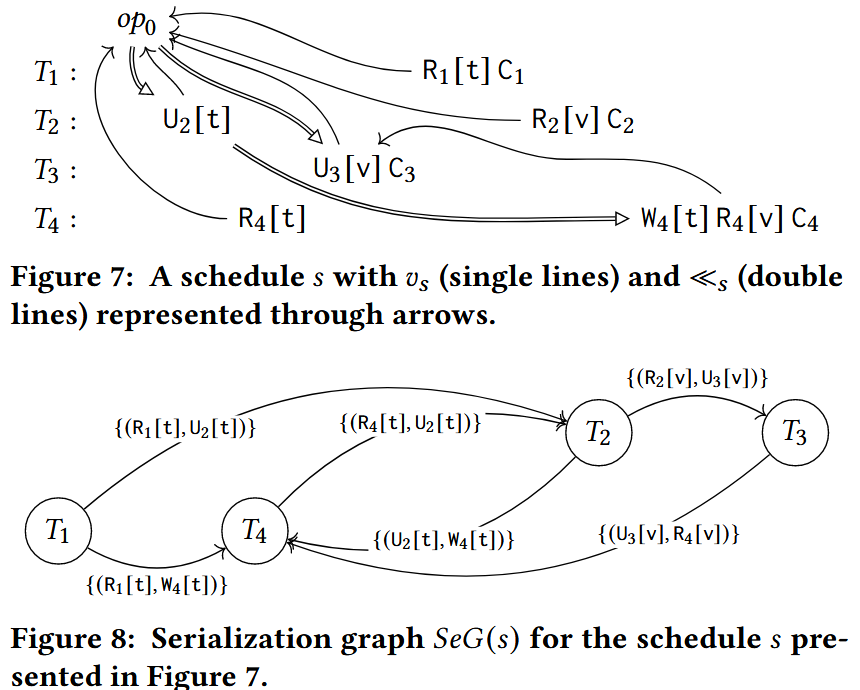
\includegraphics[width=0.98\linewidth]{figs/confliction-detect}
		\end{column}
	\end{columns}
\end{frame}
%%%%%%%%%%%%%%%%%%%%

%%%%%%%%%%%%%%%%%%%%
\begin{frame}{TODS2025 Allocating Isolation Levels to Transactions in a Multiversion Setting}

	\textbf{Limitations: }
	\begin{itemize}
		\item 依赖调度分析,不支持分布式数据库;
		\item 执行前的分析引入额外的开销;
		\item 在高度冲突的工作负载下性能优势减弱。
	\end{itemize}

\end{frame}
%%%%%%%%%%%%%%%%%%%%

%%%%%%%%%%%%%%%%%%%%
\begin{frame}{arXiv2025 2501.18377v3 Using Read Promotion and Mixed Isolation Levels for Performant Yet Serializable Execution of Transaction Programs}
	background, problems, contributions, techniques (basic ideas), limitations
\end{frame}
%%%%%%%%%%%%%%%%%%%%

%%%%%%%%%%%%%%%%%%%%
\begin{frame}{VLDB2025 TxnSails-Achieving Serializable Transaction Scheduling with Self-Adaptive Isolation Level Selection}
	background, problems, contributions, techniques (basic ideas), limitations
\end{frame}
%%%%%%%%%%%%%%%%%%%%